\documentclass[a4paper, 11pt]{article}	%Tipo de documento y opciones.

\usepackage[spanish]{babel}				%Idioma en el que se va a escibir.
\usepackage[utf8]{inputenc}				%Reconocimiento de caracteres como tildes.
\usepackage{fancyhdr}					%Paquete usado para la cabecera y el pie de página.
\usepackage{graphicx}					%Importar imágenes.
\usepackage{float}						%Posicionamiento de imágenes.

%Creamos comandos para los autores.
\newcommand{\enriquename}{Enrique Cabrerizo Fernández}
\newcommand{\guillermoname}{Guillermo Ruiz Álvarez}

\title{Práctica 3\\Redes de computadores}						%Título.
\author{\enriquename \and \guillermoname}						%Autores.
\date{14/11/2013}												%Fecha.

\pagestyle{fancyplain}					%Estilo: Usar cabeceras.
\fancyhf{}								%Borrar formato estándar.
\lhead{ \fancyplain{}{\enriquename} }	%Nombre de Enrique a la izquierda de la cabecera.
\rhead{ \fancyplain{}{\guillermoname} }	%Nombre de Guillermo a la derecha de la cabecera.
\cfoot{ \fancyplain{}{\thepage} }		%Número de la página centrada en el pie.

\begin{document}		%Comienza documento.
\maketitle			%Página de título.
\newpage				%Salto de página.
\tableofcontents		%Página de índice.
\newpage				%Salto de página.

\section{Introducción}	%Sección de introducción
En esta prática se va a implementar un programa que analizará y caracterizará una captura de paquetes de red. Para ello, utilizará un fichero \textit{*.pcap} que contenga una traza o directamente una interfaz especificada, dependiendo del argumento utilizado (véase sección \ref{sec:manual}, página \pageref{sec:manual}).
\\\\
Las funciones que realizará el programa son las siguientes:
\begin{itemize}
\item Mostrar por pantalla los porcentajes de paquetes IP, no ETH-IP, TCP, UDP y no TCP-UDP.
\item Mostrar por pantalla el top de 5 direcciones IP activas y el top de 5 puertos activos  (ambos por paquetes y tamaño en bytes).
\item Almacene en fichero y calcule el ECDF de la variable \textit{tamaño de paquete capturado}.
\item Almacene en fichero el ancho de banda a nivel 2 cada segundo por sentido.
\item Almacene en fichero y calcule el ECDF de la variable \textit{tiempo entre llegadas de los paquetes de un flujo entre un par de puertos}.
\end{itemize}

Adicionalmente se calcularán histogramas de las variables en las que se pide calcular un ECDF, para así disponer de más información para analizar los datos.

De forma particular, el análisis que se va a llevar a cabo consistirá en mostrar la funcionalidad de la herramienta sobre el fichero proporcionado con el enunciado de la práctica: \textit{$practica3\_ rc1lab.pcap$}

\section{Análisis de la traza}
\subsection{Porcentajes de protocolos}
En la \textbf{Figura \ref{fig:recuento}} se muestran los porcentajes de los paquetes IP, no Eth-IP, UDP, TCP y no UDP-TCP.

%Inclusion de imagen.
\begin{figure}[H]
\centering
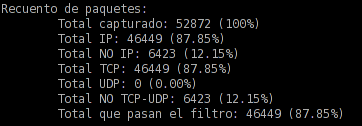
\includegraphics[width=0.8\textwidth]{recuento.png}
\caption{Recuento y porcentajes de protocolos de paquetes.}
\label{fig:recuento}
\end{figure}

Se puede observar que el $12,15\%$ de los paquetes (6423 paquetes) no son Eth-IP. Un análisis posterior con Wireshark nos dirá que su tipo de ethernet corresponde a \textit{802.1Q Virtual LAN (0x8100)}.

El resto de paquetes son todos TCP/IP, los dos protocolos más importantes del conjunto de protocolos de internet.

El campo \textit{Total que pasan el filtro} cuenta aquellos paquetes que pasan el filtro especificado mediante los argumentos. El filtro básico, para el que no se utiliza ningún argumento adicional, es que el paquete sea Eth-IP.

\subsection{Popularidad de direcciones IP y puertos}
En la \textbf{Figura \ref{fig:popIP}} se muestra el top 5 de direcciones IP activas y en la \textbf{Figura \ref{fig:popPuertos}} se muestra el top 5 de puertos activos, ambos clasificados por \textit{número de paquetes, tamaño en bytes, origen} y \textit{destino}.

%Inclusion de imagen.
\begin{figure}[H]
\centering
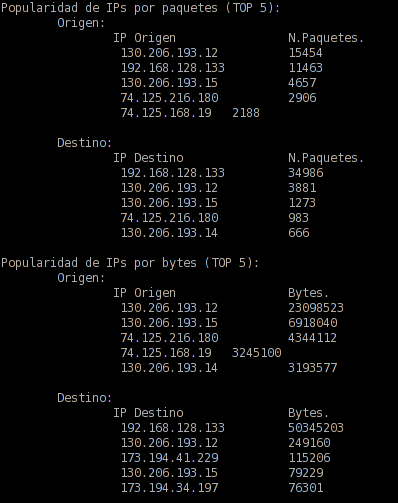
\includegraphics[width=0.8\textwidth]{popularidadIP.png}
\caption{Popularidad de direcciones IP.}
\label{fig:popIP}
\end{figure}

La razón por la cual las clasificaciones por paquetes no coinciden con las clasificaciones por tamaños es que muchos de los paquetes enviados o recibidos por algunas direcciones o puertos son asentimientos (ACK). Por tanto, aunque una dirección o puerto pueda recibir o enviar muchos paquetes, si un porcentaje elevado de estos son asentimientos sólo ocuparan 54 bytes (el tamaño mínimo de una trama ethernet), es decir, que se habrán enviado o recibido muchos paquetes pero de poco tamaño.

%Inclusion de imagen.
\begin{figure}[H]
\centering
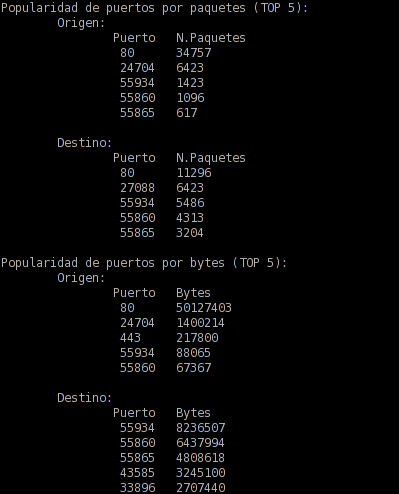
\includegraphics[width=0.8\textwidth]{popularidadPuertos.png}
\caption{Popularidad de puertos.}
\label{fig:popPuertos}
\end{figure}

\subsection{Tamaños de los paquetes}
Para analizar la variable \textit{tamaño del paquete capturado} se han realizado un histograma y un ECDF de dicha variable sobre la traza. (Véase figura XXXXXXXXXXXXX).

\subsection{Ancho de banda a nivel 2}
Se analizará el ancho de banda a nivel 2 cada segundo por sentido asumiendo que la dirección Ethernet origen es \textit{00:55:22:af:c6:37} y descartando el tráfico broadcast.

\subsection{Tiempo entre llegadas de paquetes de un flujo}
Para analizar los tiempos entre llegadas de paquetes de un flujo, se asumirá el flujo UDP con puertos de origen y destino 24704 y 27088 respectivamente. Dicho análisis se llevará a cabo con la ayuda de Wireshark dado que la pila de protocolos usada no es Eth-IP, sino VLAN.

%Apendice
\clearpage
\appendix
\renewcommand\appendixname{Anexo}
\section{Manual de utilización del programa}
\label{sec:manual}
En esta sección se ofrece una breve explicación sobre la utilización del programa implementado.
\subsection{Compilación}
Para compilar el programa se proporciona un fichero Makefile, existen tres opciones equivalentes para la compilación del mismo utilizando el programa make:
\begin{itemize}
\item \textbf{make all} compila el programa y le da el nombre \textit{practica3}
\item \textbf{make practica3} compila el programa y le da el nombre \textit{practica3}
\item \textbf{make main} compila el programa y le da el nombre \textit{main}
\end{itemize}

Para limpiar los archivos generados por la compilación, basta con ejecutar \textbf{make clean}.

\subsection{Ejecución}
Para ejecutar el programa se utiliza la siguiente estructura:

\begin{center}
\textbf{./practica3 INTERF $[<$filtro$>$ $<$dato a filtrar$>]$}
\end{center}

\noindent Donde:\\
\textbf{INTERF} es el fichero pcap o interfaz ethernet (ethX con $X \in [0,9]$).\\
\textbf{$[<$filtro$>$ $<$dato a filtrar$>]:$} puede ser:\\
\indent -ipo x.x.x.x : filtro de IP de origen x.x.x.x ($x \in [0, 255]$)\\
\indent -ipd x.x.x.x : filtro de IP de destino x.x.x.x ($x \in [0, 255]$)\\
\indent -po x : filtro de puerto de origen x ($x \in [0,65536]$)\\
\indent -pd x : filtro de puerto de destino x ($x \in [0,65536]$)\\
\indent -etho xx:xx:xx:xx:xx:xx : filtro de MAC origen ($xx \in [00,FF]$)\\
\indent -ethd xx:xx:xx:xx:xx:xx : filtro de MAX destino ($xx \in [00,FF]$)\\

Se pueden aplicar varios filtros a la vez y el orden de los mismos no se tiene en cuenta.
Si un filtro IP es 0.0.0.0, un filtro de puertos es 0, o un filtro ethernet es 00:00:00:00:00:00 se considerará inexistente, es decir, no se aplicará dicho filtro.

\end{document}